\section{Server architecture}
\label{sec:arch_server}
The server is the systems back-end it is responsible for permanently storing data and providing it to the user on demand. The team decided that the server should be RESTful in order to make it easy to access. The data-interchange format chosen to transfer data between the app and the server is JSON. This format was chosen for its human readability and it is also very easily parsed by computer software. In addition, both these properties allow for easy integration with future functionality.

\subsection{Dropwizard}
The server is implemented in Dropwizard which is a Java framework for making RESTful web services. Dropwizard was chosen for its use of popular Java libraries such as Jetty, Jersey, and Jackson to implement its functionality. The main class of the server is a service that at runtime provides access to the database and adds resources to the runtime environment. The main structure of how the server uses resources and the database can be found in figure~\ref{fig:classDiagramServer}.

\begin{figure}[H]
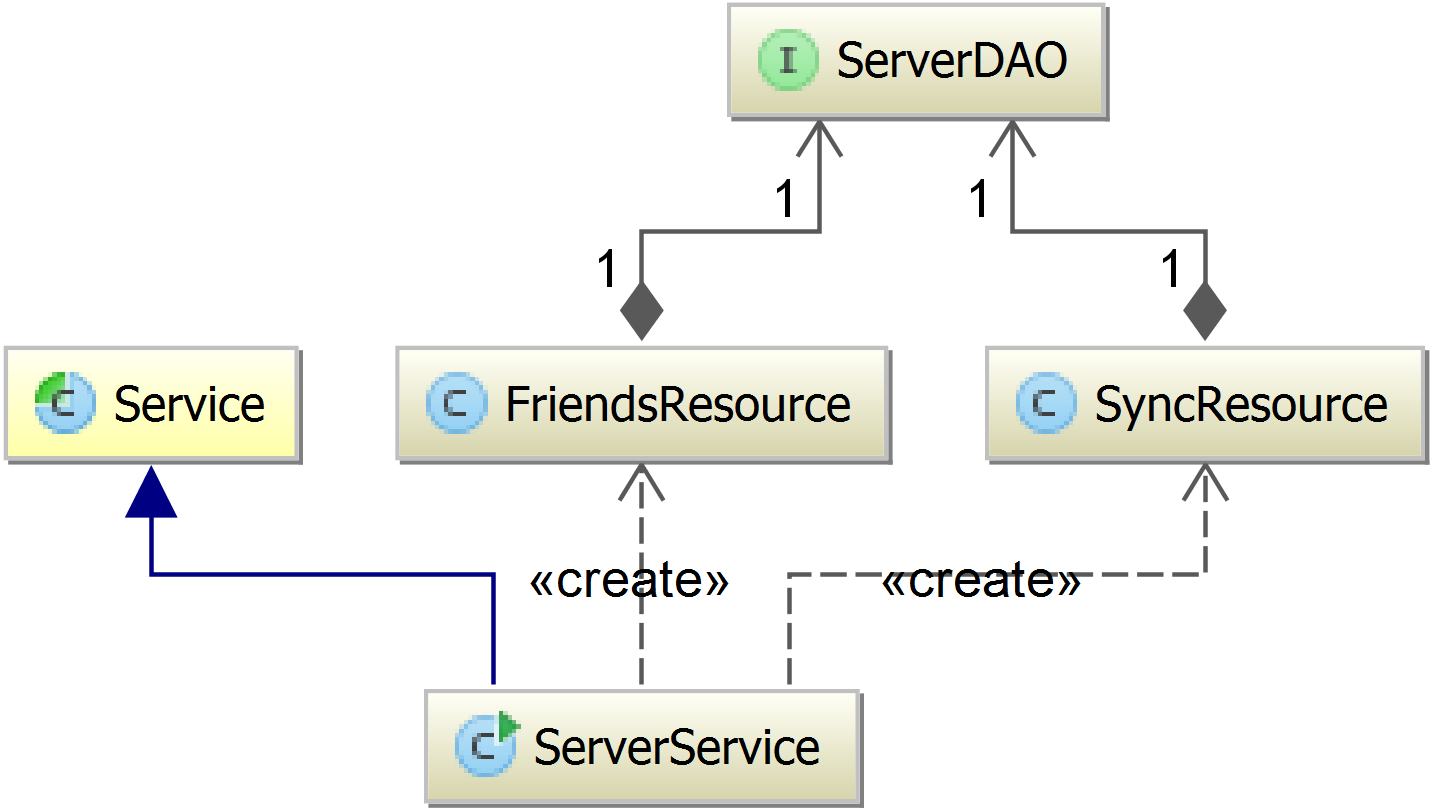
\includegraphics[width=\textwidth]{ch/architecture/fig/classDiagramServer.png}
\caption{Class diagram for main server structure}
\label{fig:classDiagramServer}
\end{figure}

\subsubsection{Resources}
A Dropwizard implementation has a set of resource classes. These classes contain methods that map to a URI path. When the server receives a HTTP request it will try the match the path to the paths defined by the resource methods, it will then call the method found or return a 404 Not Found error. An example resource class is included in code~\ref{lst:dropwizardResource}. The method in this resource will handle HTTP GET calls to /user/{user}/sync/usage/{timestamp} where {user} and {timestamp} matches any text. These variables is then used inside the method to perform actions depending on user and time stamp.

\noindent\begin{minipage}{\textwidth}
\begin{lstlisting}[caption={Dropwizard resource example}, label={lst:dropwizardResource}]
@Path("user/{user}/sync")
@Produces(MediaType.APPLICATION_JSON)
public class SyncResource {
    @GET
    @Path("/usage/{timestamp}")
    public List<DeviceUsage> getUpdatedUsage(
	   @PathParam("timestamp") LongParam timestamp, 
	   @PathParam("user") LongParam userId) {
        List<DeviceUsage> usage = db.getUpdatedUsage(
		       userId.get(), timestamp.get());
        if(usage != null && !usage.isEmpty())
            return usage;
        else
            throw new WebApplicationException(
			         Response.Status.NO_CONTENT);
    }
}
\end{lstlisting}
\end{minipage}

\subsubsection{Database abstraction}
Dropwizard uses the JDBC and JDBI libraries to communicate with the database. The JDBC library is Javas standard interface to databases. MySQL provides a driver for JDBC in order to make communication possible. JDBI is a convenience layer on top of JDBC which makes it possible to write an interface with SQL queries and use that interface as a data access object.

\subsection{Database}
For permanent storage the server uses MySQL. MySQL is a reliable and easy to set up database. A diagram of how the database is designed can be found in figure~\ref{fig:ER-Diagram}

\begin{figure}[H]
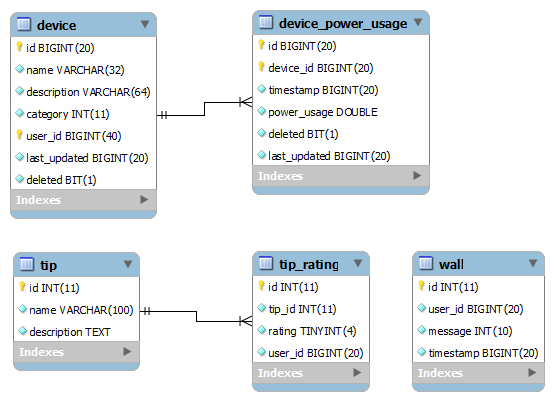
\includegraphics[width=\textwidth]{ch/architecture/fig/ER-Diagram.png}
\caption{ER-Diagram for the database}
\label{fig:ER-Diagram}
\end{figure}
